\section{实验:用安培表测电流强度}\label{sec:8-2}

这个实验的目的是练习正确使用安培表。
我们用安培表先测图 \ref{fig:8-3} 甲所示电路中的电流强度,再测图乙所示电路中的电流强度。
列出实验需要的器材清单,再接清单检查实验桌上的器材是否够用。

\begin{figure}[H]
    \centering
    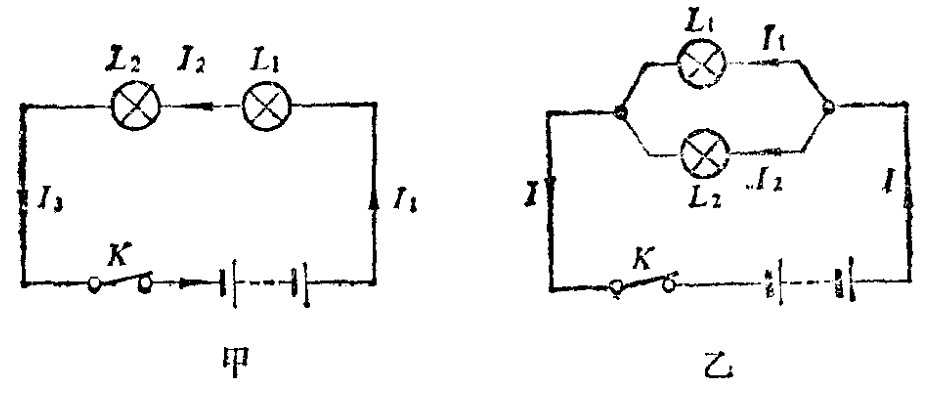
\includegraphics[width=0.7\textwidth]{../pic/czwl2-ch8-3}
    \caption{}\label{fig:8-3}
\end{figure}

学生实验最常用的安培表,是有三个接线柱、两个量程的安培表。
一种如图 \ref{fig:8-4} 以甲所示,还有一种如图 \ref{fig:8-4} 乙所示。
\begin{figure}[htbp]
    \centering
    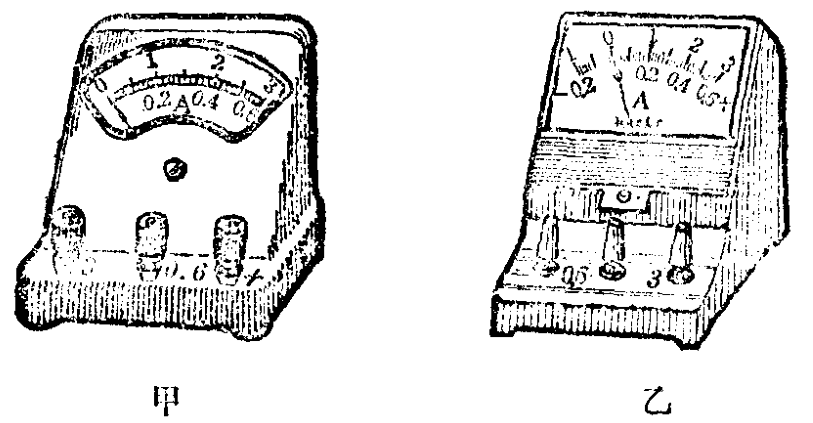
\includegraphics[width=0.7\textwidth]{../pic/czwl2-ch8-4}
    \caption{有两个量程的安培表}\label{fig:8-4}
\end{figure}
图 \ref{fig:8-4} 甲所示的安培表,两个量程共用一个“$+$” 接线柱,标着 “0.6” 与 “3” 的为负接线柱。
当使用标着 “$+$” 和 “0.6” 这两个接线柱的时候,量程是 0.6 安培,刻度盘上每个大格是 0.2 安培,每个小格是 0.02 安培。
当使用 “$+$” 和 “3” 这两个接线柱的时候,量程是 3 安培,每个大格是 1 安培,每个小格是 0.1 安培。
图 \ref{fig:8-4} 乙所示的安培表,两个量程共用一个 “$-$” 接线柱,标着 “0.6” 与 “3” 的为正接线柱。
这种安培表刻度盘 “0” 点的位置不在最左端,“0” 点左侧还有一些刻度。

在练习使用安培表以前,先要仔细观察所用的安培表,看看它有几个量程,
各是多少安培,弄清刻度盘上每个大格和每个小格的安培数。
然后检查指针是否对准零刻度,如果没有对准,可请老师帮助校正。

这个实验是初次使用安培表,为了避免接错,每次测量前要先画好电路图,
在图中安培表符号两侧标上 “$+$”、“$-$” 号代表它的两个接线柱,
经小组同学认真检查,一致认为正确以后,再按图连接。
为了避免电流过强损坏安培表,在不能预先估算电流强度的情况下,
要先拿电路的一个线头迅速试触最大量程的接线柱,
如果指针示数在较小的量程的范围内,再使用较小的量程(想想看,这有什么好处)。

照图 \ref{fig:8-3} 甲把电池组、电键、小灯泡 $L_1$ 和 $L_2$ 串联起来。
用安培表先测电池组正极和 $L_1$ 间的电流强度 $I_1$,
再依次测出 $L_1$ 和 $L_2$ 间、$L_2$ 和电池组负极间的电流强度 $I_2$、$L_3$。
把测得的值记下来。

根据测得的 $I_1$、$I_2$、$I_3$ 的值回答:串联电路中各处的电流强度是不是相等?
测串联电路的电流强度的时候,电流表连入的位置对测量结果有没有影响?

照图 \ref{fig:8-3} 乙组成并联电路,用安培表依次测出
$L_1$ 支路的电流 $I_1$, $L_2$ 支路的电流 $I_2$,干路的电流 $I$。
把测得的值记下来。

根据测得的值回答:并联电路中各支路的电流强度和干路的电流强度是否相同?
各支路的电流强度之和跟干路的电流强度有什么关系?


\lianxi

(1) 每秒钟通过电子手表、晶体管电视机、汽车发电机的电量,各约多少库仑?

(2) 在 1 分钟内有 18 库仑的电量通过手电筒的小灯泡,求小灯泡中的电流强度。

(3) 一盏电灯的电流强度是 300 毫安,合多少安培?5 分钟通过它的电量是多少库仑?

(4) 在图 \ref{fig:8-5} 里,要用安培表量度小灯泡的电流强度,估计电流强度大约是 0.8 安培,
那么电路的两个线头 $A$、$B$ 各应接在安培表的哪个接线柱上?

\begin{figure}[htbp]
    \centering
    \begin{minipage}{7cm}
    \centering
    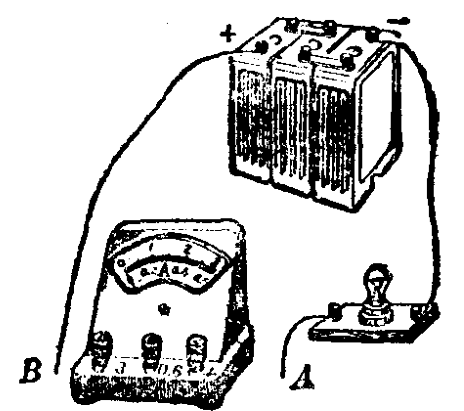
\includegraphics[width=6cm]{../pic/czwl2-ch8-5}
    \caption{}\label{fig:8-5}
    \end{minipage}
    \qquad
    \begin{minipage}{7cm}
    \centering
    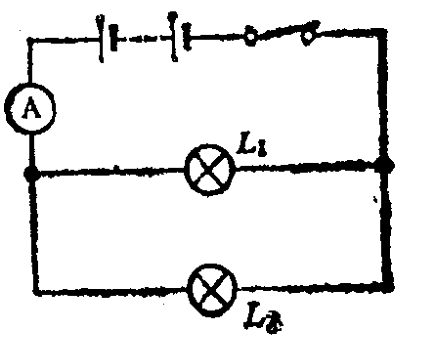
\includegraphics[width=6cm]{../pic/czwl2-ch8-6}
    \caption{}\label{fig:8-6}
    \end{minipage}
\end{figure}

(5) 在图 \ref{fig:8-6} 中, 通过电灯 $L_1$ 的电流强度是 0.4 安培,通过电灯 $L_2$ 的电流强度是 0.6 安培。
那么干路中的电流强度是多少安培?图中安培表的示数是多少?

(6) 图 \ref{fig:8-7} 是一只安培表的刻度盘。图甲是当电路的两个线头接在 “$+$” 和 “3” 两个接线柱上时,指针的位置。
图乙是对另一个电路测量,电路的两个线头接在 “$+$” 和 “0.6” 两个接线柱上时,指针的位置。
这两次测得的电流强度各是多大?

\begin{figure}[htbp]
    \centering
    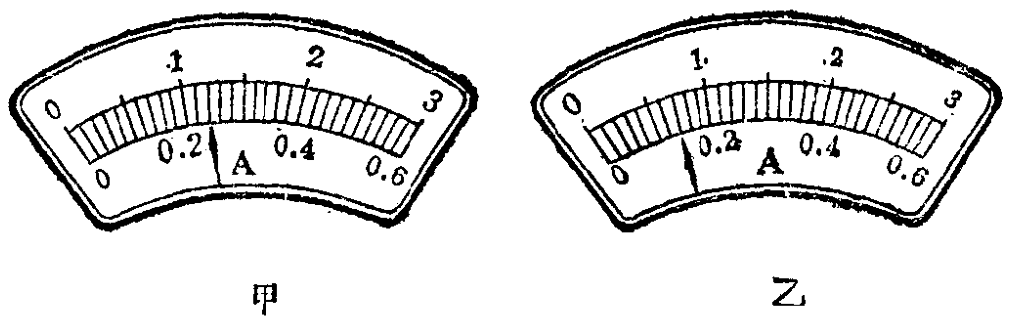
\includegraphics[width=0.7\textwidth]{../pic/czwl2-ch8-7}
    \caption{}\label{fig:8-7}
\end{figure}

